\chapter{\RU{Поиск нужных инструкций}\EN{Finding the right instructions}}

\RU{Если программа использует инструкции сопроцессора, и их не очень много, 
то можно попробовать вручную проверить отладчиком какую-то из них.}
\EN{If the program is utilizing FPU instructions and there are very few of them in the code,
one can try to check each one manually with a debugger.}\\
\\
\RU{К примеру, нас может заинтересовать, при помощи чего Microsoft Excel считает 
результаты формул, введенных пользователем. Например, операция деления.}
\EN{For example, we may be interested how Microsoft Excel calculates the formulae entered by user.
For example, the division operation.}

\index{\GrepUsage}
\index{x86!\Instructions!FDIV}
\RU{Если загрузить excel.exe (из Office 2010) версии 14.0.4756.1000 в \IDA, затем сделать полный листинг 
и найти все инструкции \FDIV (но кроме тех, которые в качестве второго операнда используют константы ~--- они, 
очевидно, не подходят нам):}
\EN{If we load excel.exe (from Office 2010) version 14.0.4756.1000 into \IDA, make a full listing
and to find every \FDIV instruction (except the ones which use constants as a second 
operand~---obviously, they do not suit us):}\\

\begin{lstlisting}
cat EXCEL.lst | grep fdiv | grep -v dbl_ > EXCEL.fdiv
\end{lstlisting}

\RU{\dots то окажется, что их всего 144.}\EN{\dots then we see that there are 144 of them.}\\
\\
\RU{Мы можем вводить в Excel строку вроде \TT{=(1/3)} и проверить все эти инструкции.}
\EN{We can enter a string like \TT{=(1/3)} in Excel and check each instruction.}\\
\\
\index{tracer}
\RU{Проверяя каждую инструкцию в отладчике или \tracer 
(проверять эти инструкции можно по 4 за раз), 
окажется, что нам везет и срабатывает всего лишь 14-я по счету:}
\EN{By checking each instruction in a debugger or \tracer
(one may check 4 instruction at a time),
we get lucky and the sought-for instruction is just the 14th:}

\begin{lstlisting}
.text:3011E919 DC 33                                fdiv    qword ptr [ebx]
\end{lstlisting}

\begin{lstlisting}
PID=13944|TID=28744|(0) 0x2f64e919 (Excel.exe!BASE+0x11e919)
EAX=0x02088006 EBX=0x02088018 ECX=0x00000001 EDX=0x00000001
ESI=0x02088000 EDI=0x00544804 EBP=0x0274FA3C ESP=0x0274F9F8
EIP=0x2F64E919
FLAGS=PF IF
FPU ControlWord=IC RC=NEAR PC=64bits PM UM OM ZM DM IM 
FPU StatusWord=
FPU ST(0): 1.000000
\end{lstlisting}

\RU{В \ST{0} содержится первый аргумент (1), второй содержится в}
\EN{\ST{0} holds the first argument (1) and second one is in} \TT{[EBX]}.\\
\\
\index{x86!\Instructions!FDIV}
\RU{Следующая за \FDIV инструкция (\TT{FSTP}) записывает результат в память:}
\EN{The instruction after \FDIV (\TT{FSTP}) writes the result in memory:}\\

\begin{lstlisting}
.text:3011E91B DD 1E                                fstp    qword ptr [esi]
\end{lstlisting}

\RU{Если поставить breakpoint на ней, то мы можем видеть результат:}
\EN{If we set a breakpoint on it, we can see the result:}

\begin{lstlisting}
PID=32852|TID=36488|(0) 0x2f40e91b (Excel.exe!BASE+0x11e91b)
EAX=0x00598006 EBX=0x00598018 ECX=0x00000001 EDX=0x00000001
ESI=0x00598000 EDI=0x00294804 EBP=0x026CF93C ESP=0x026CF8F8
EIP=0x2F40E91B
FLAGS=PF IF
FPU ControlWord=IC RC=NEAR PC=64bits PM UM OM ZM DM IM 
FPU StatusWord=C1 P 
FPU ST(0): 0.333333
\end{lstlisting}

\RU{А также, в рамках пранка\footnote{practical joke}, модифицировать его на лету:}
\EN{Also as a practical joke, we can modify it on the fly:}\\

\begin{lstlisting}
tracer -l:excel.exe bpx=excel.exe!BASE+0x11E91B,set(st0,666)
\end{lstlisting}

\begin{lstlisting}
PID=36540|TID=24056|(0) 0x2f40e91b (Excel.exe!BASE+0x11e91b)
EAX=0x00680006 EBX=0x00680018 ECX=0x00000001 EDX=0x00000001
ESI=0x00680000 EDI=0x00395404 EBP=0x0290FD9C ESP=0x0290FD58
EIP=0x2F40E91B
FLAGS=PF IF
FPU ControlWord=IC RC=NEAR PC=64bits PM UM OM ZM DM IM 
FPU StatusWord=C1 P 
FPU ST(0): 0.333333
Set ST0 register to 666.000000
\end{lstlisting}

\RU{Excel показывает в этой ячейке $666$, что окончательно убеждает нас в том, что мы нашли нужное место.}
\EN{Excel shows $666$ in the cell, finally convincing us that we have found the right point.}

\begin{figure}[H]
\centering
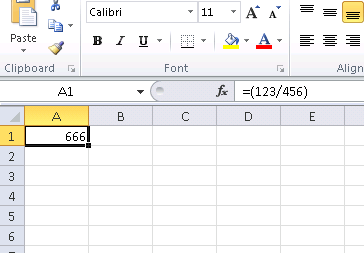
\includegraphics[scale=\NormalScale]{digging_into_code/Excel_prank.png}
\caption{\RU{Пранк сработал}\EN{The practical joke worked}}
\end{figure}

\RU{Если попробовать ту же версию Excel, только x64, то окажется что там инструкций \FDIV всего 12, 
причем нужная нам ~--- третья по счету.}
\EN{If we try the same Excel version, but in x64,
we will find only 12 \FDIV instructions there,
and the one we looking for is the third one.}

\begin{lstlisting}
tracer.exe -l:excel.exe bpx=excel.exe!BASE+0x1B7FCC,set(st0,666)
\end{lstlisting}

\index{x86!\Instructions!DIVSD}
\RU{Видимо, все дело в том, что много операций деления переменных типов \Tfloat и \Tdouble 
компилятор заменил на SSE-инструкции вроде \TT{DIVSD}, 
коих здесь теперь действительно много (\TT{DIVSD} присутствует в количестве 268 инструкций).}
\EN{It seems that a lot of division operations of \Tfloat and \Tdouble types, were replaced by the compiler with SSE instructions
like \TT{DIVSD} (\TT{DIVSD} is present 268 times in total).}
